\subsection{\(\beta\)ショックのグラフ}
\label{sec:chapter5_beta_shock_graphs}
まずは主要な変数のインパルス応答グラフを以下に提示する。
「自国の効用\(u^H\)と厚生\(W^H\)」のうち\(\Delta\)無しと書かれているものは
\ref{sec:chapter5_welfare}
節の補正がおこなわれておらず、\(\Delta\)有りと書かれているものは補正がおこなわれている。
\begin{figure}[H]
    \centering
    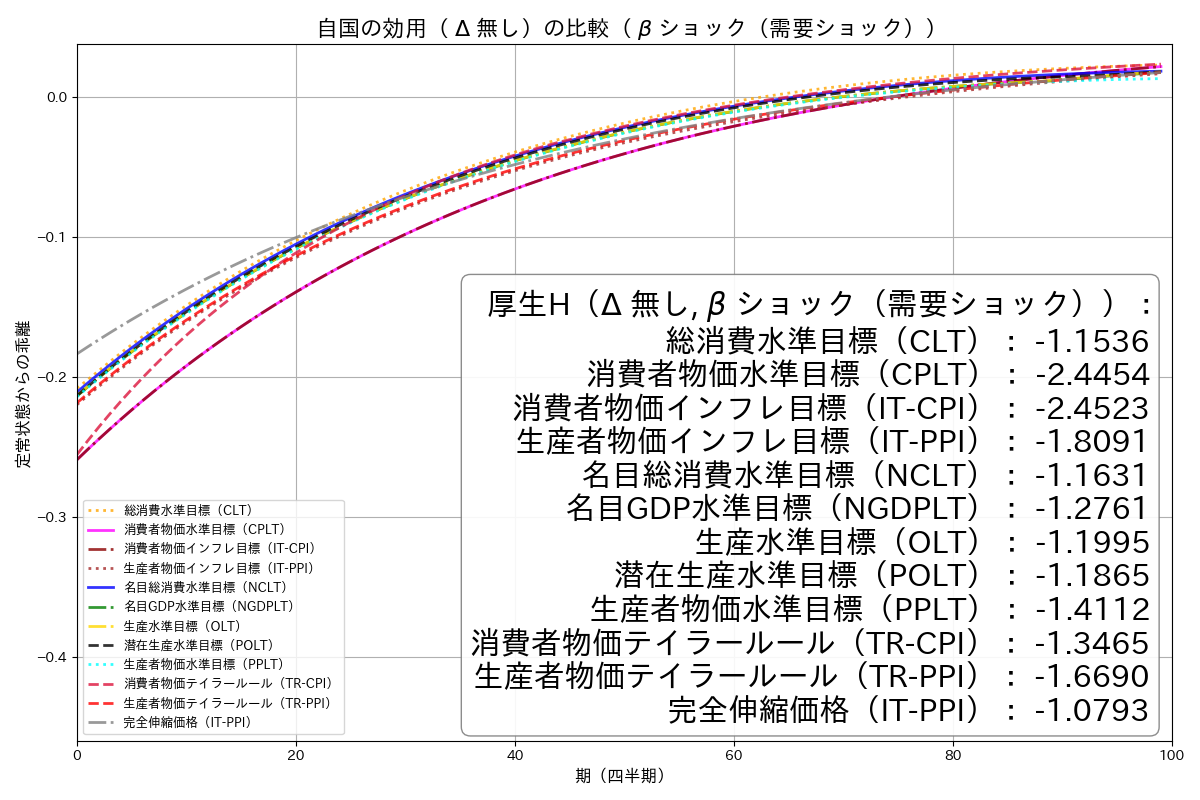
\includegraphics[width=0.9\textwidth]{comparison_graphs/beta_shock/beta_shock_utility_H_without_delta.png}
    \caption{自国の効用\(u^H\)と厚生\(W^H\)（\(\Delta\)無し）}
    \label{fig:chapter5_beta_shock_graphs_utility_H_without_delta}
\end{figure}
\begin{figure}[H]
    \centering
    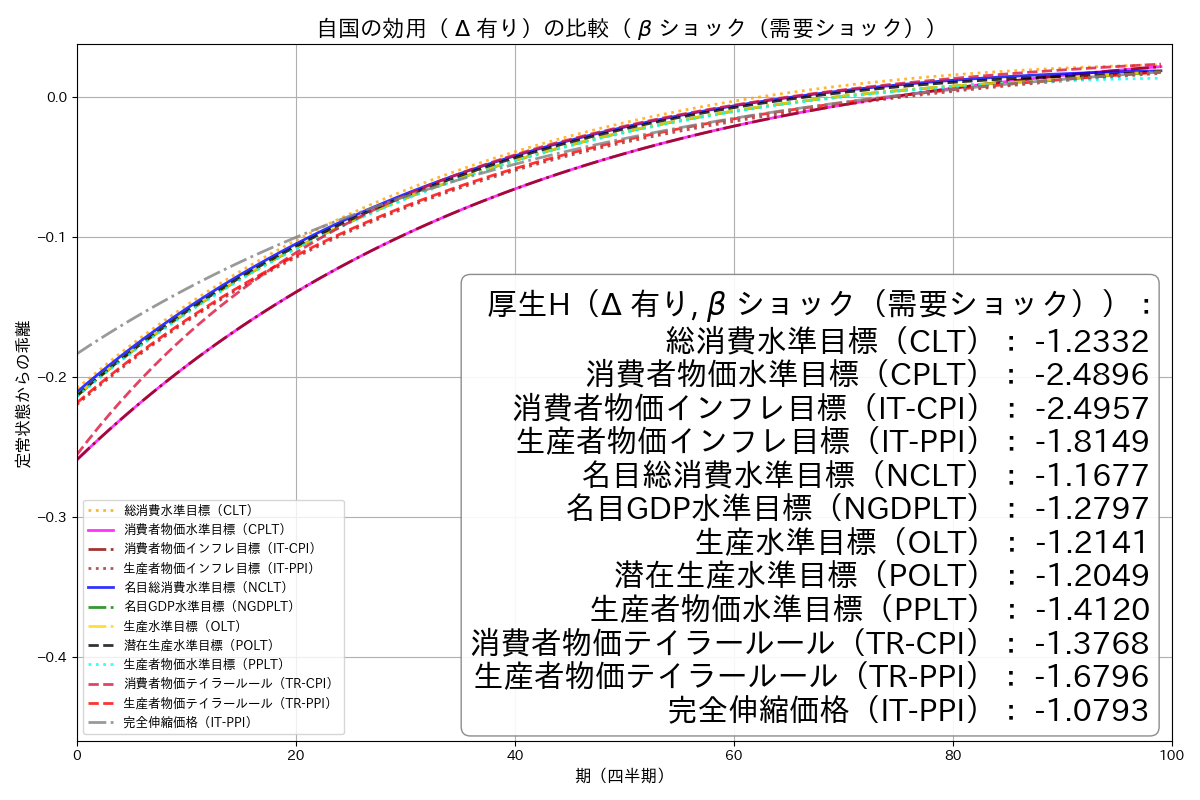
\includegraphics[width=0.9\textwidth]{comparison_graphs/beta_shock/beta_shock_utility_H_with_delta.png}
    \caption{自国の効用\(u^H\)と厚生\(W^H\)（\(\Delta\)有り）}
    \label{fig:chapter5_beta_shock_graphs_utility_H_with_delta}
\end{figure}
\begin{figure}[H]
    \centering
    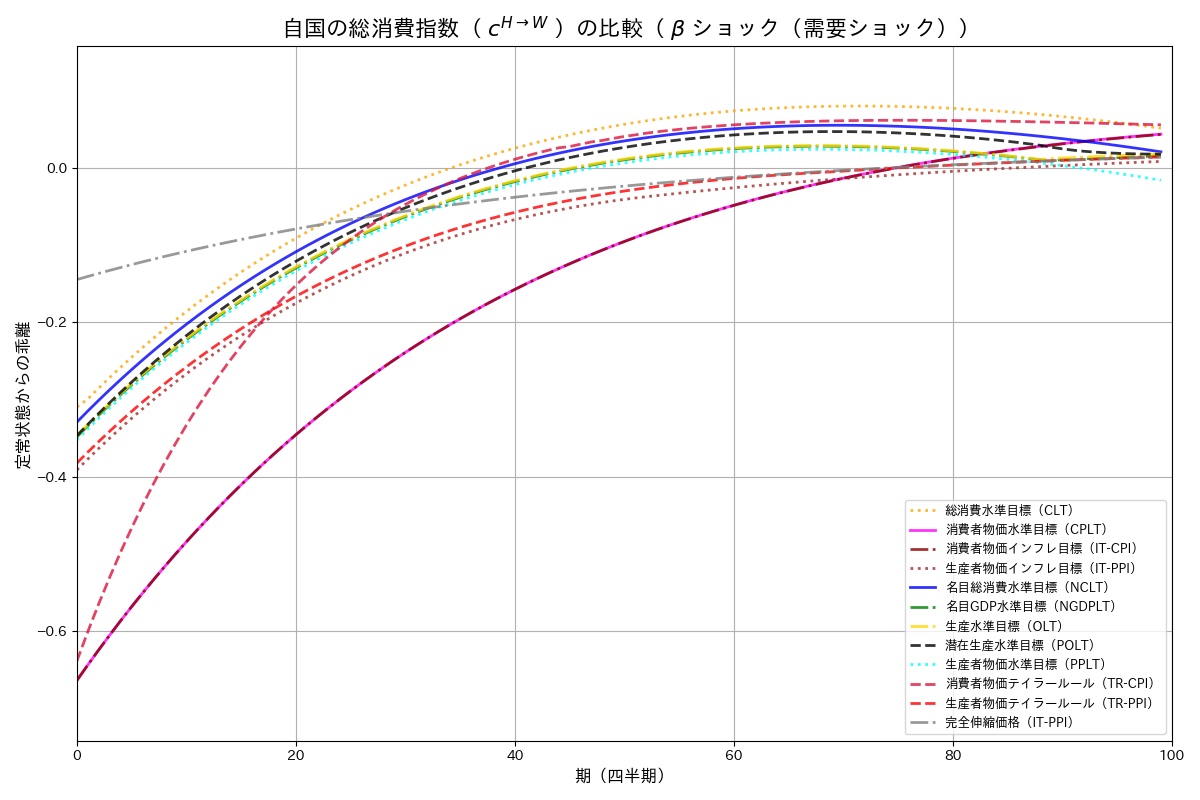
\includegraphics[width=0.9\textwidth]{comparison_graphs/beta_shock/beta_shock_c_H_W.png}
    \caption{自国の総消費指数\(c^{H\to W}\)}
    \label{fig:chapter5_beta_shock_graphs_c_H_W}
\end{figure}
\begin{figure}[H]
    \centering
    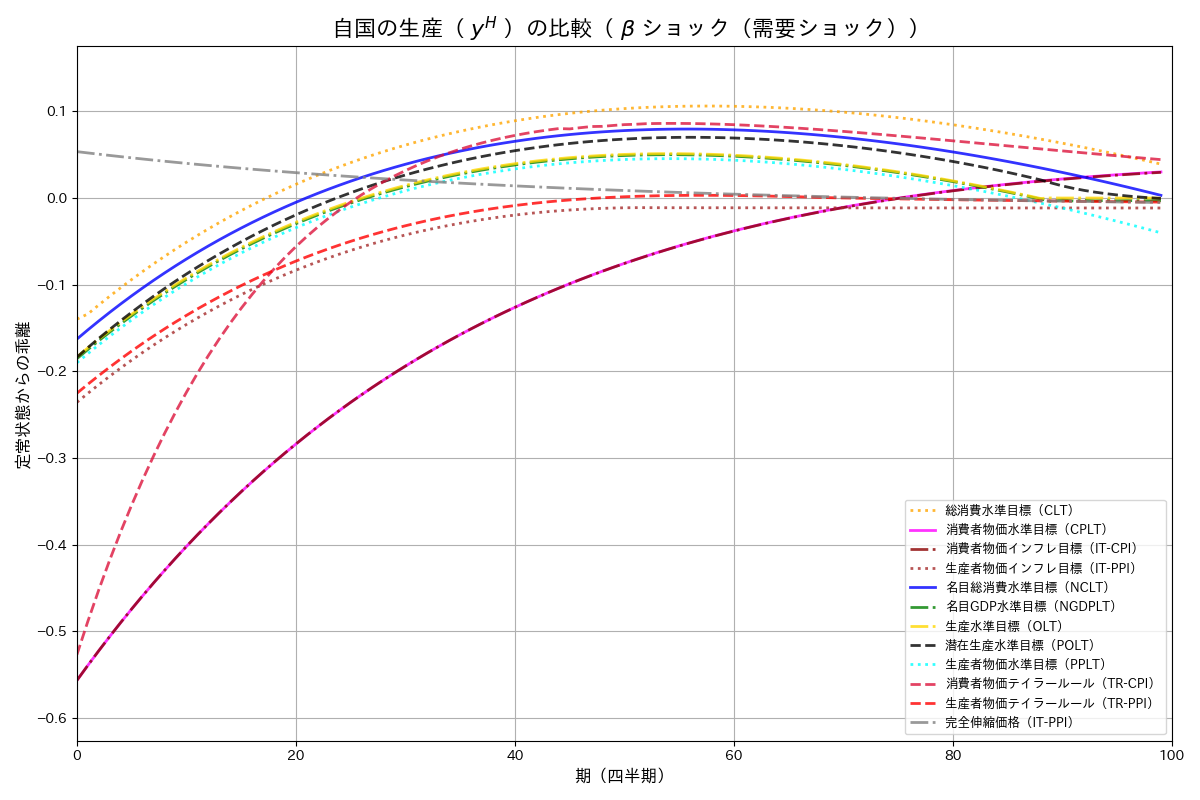
\includegraphics[width=0.9\textwidth]{comparison_graphs/beta_shock/beta_shock_y_H.png}
    \caption{自国の生産\(y^H\)}
    \label{fig:chapter5_beta_shock_graphs_y_H}
\end{figure}
\begin{figure}[H]
    \centering
    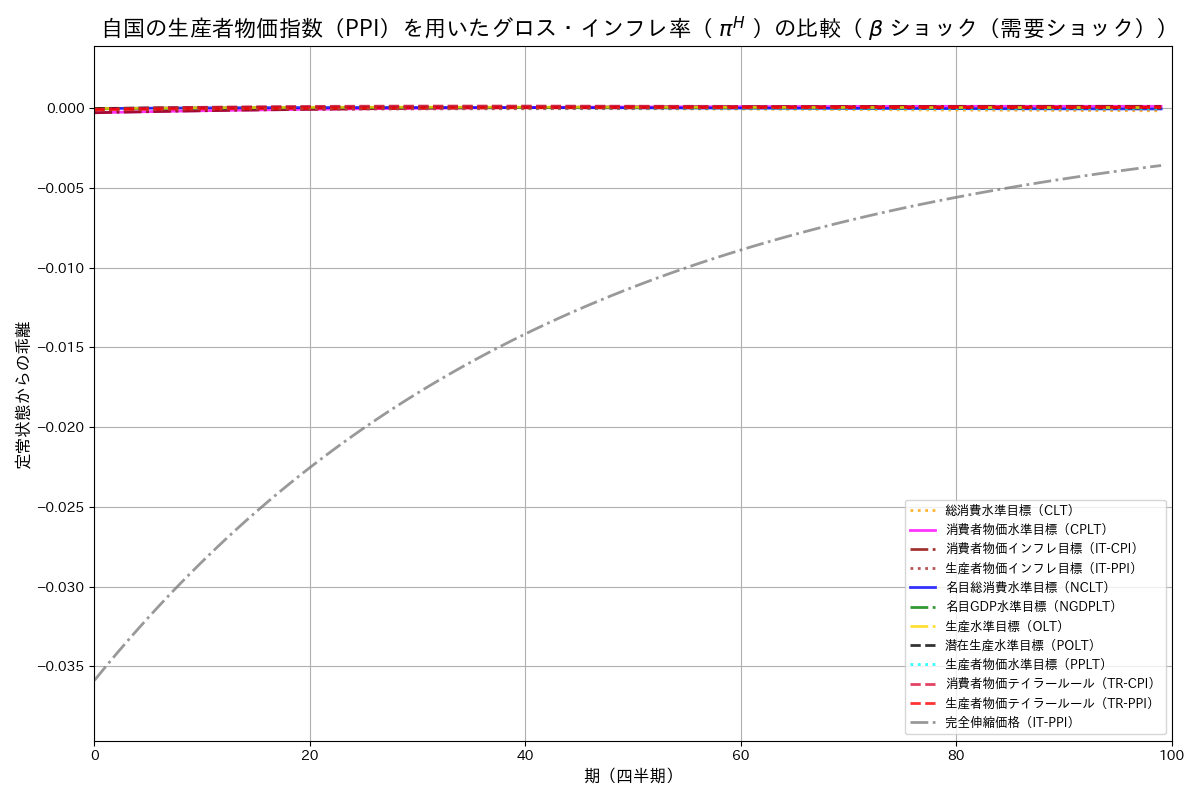
\includegraphics[width=0.9\textwidth]{comparison_graphs/beta_shock/beta_shock_pi_H.png}
    \caption{自国の生産者物価指数（PPI）を用いたグロス・インフレ率\(\pi^H\)}
    \label{fig:chapter5_beta_shock_graphs_pi_H}
\end{figure}
\begin{figure}[H]
    \centering
    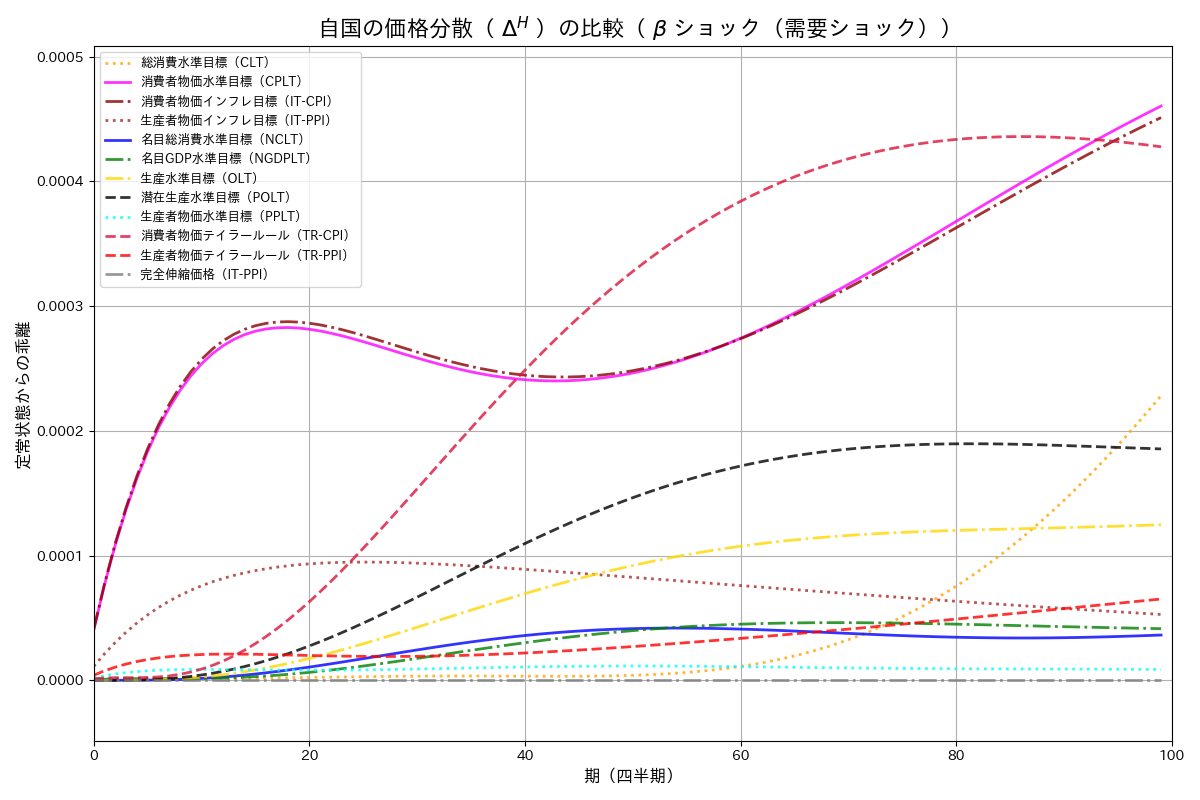
\includegraphics[width=0.9\textwidth]{comparison_graphs/beta_shock/beta_shock_Delta_H.png}
    \caption{価格分散\(\Delta_t^H\)}
    \label{fig:chapter5_beta_shock_graphs_Delta_H}
\end{figure}
\begin{figure}[H]
    \centering
    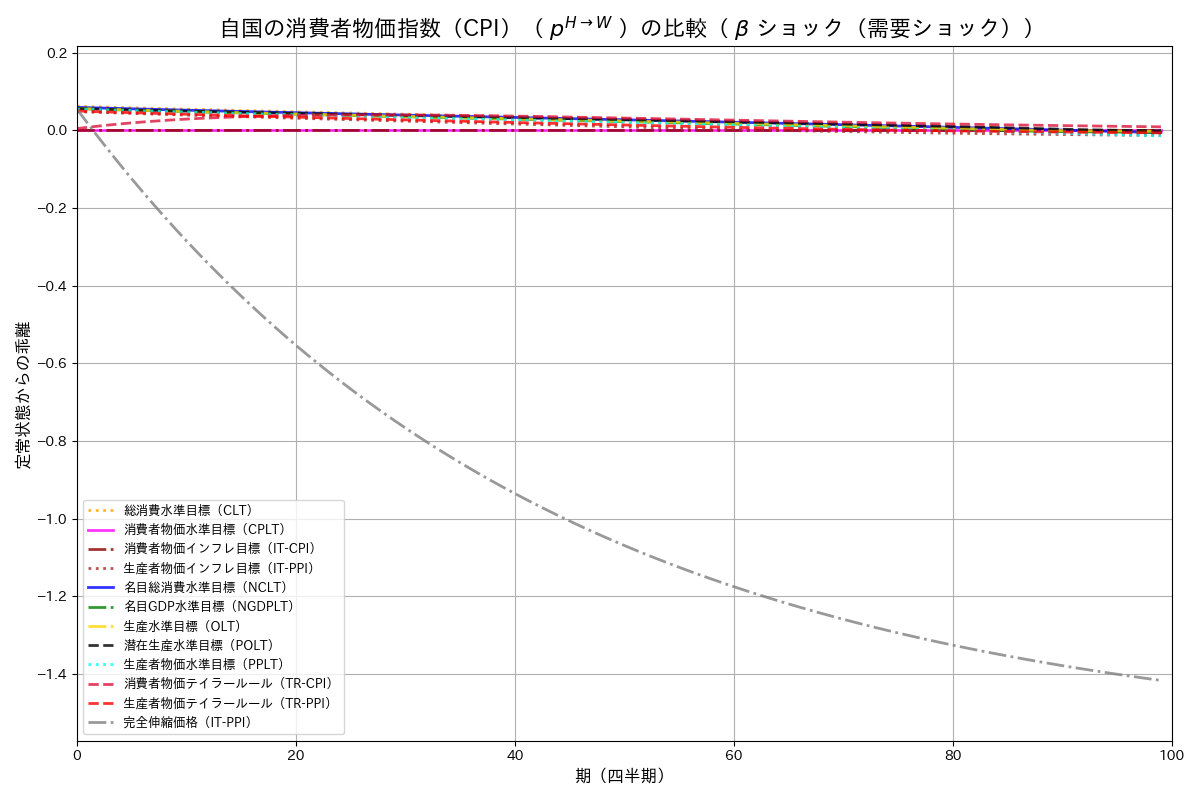
\includegraphics[width=0.9\textwidth]{comparison_graphs/beta_shock/beta_shock_p_H_W.png}
    \caption{自国の消費者物価指数（CPI）\(p^{H\to W}\)}
    \label{fig:chapter5_beta_shock_graphs_p_H_W}
\end{figure}
\begin{figure}[H]
    \centering
    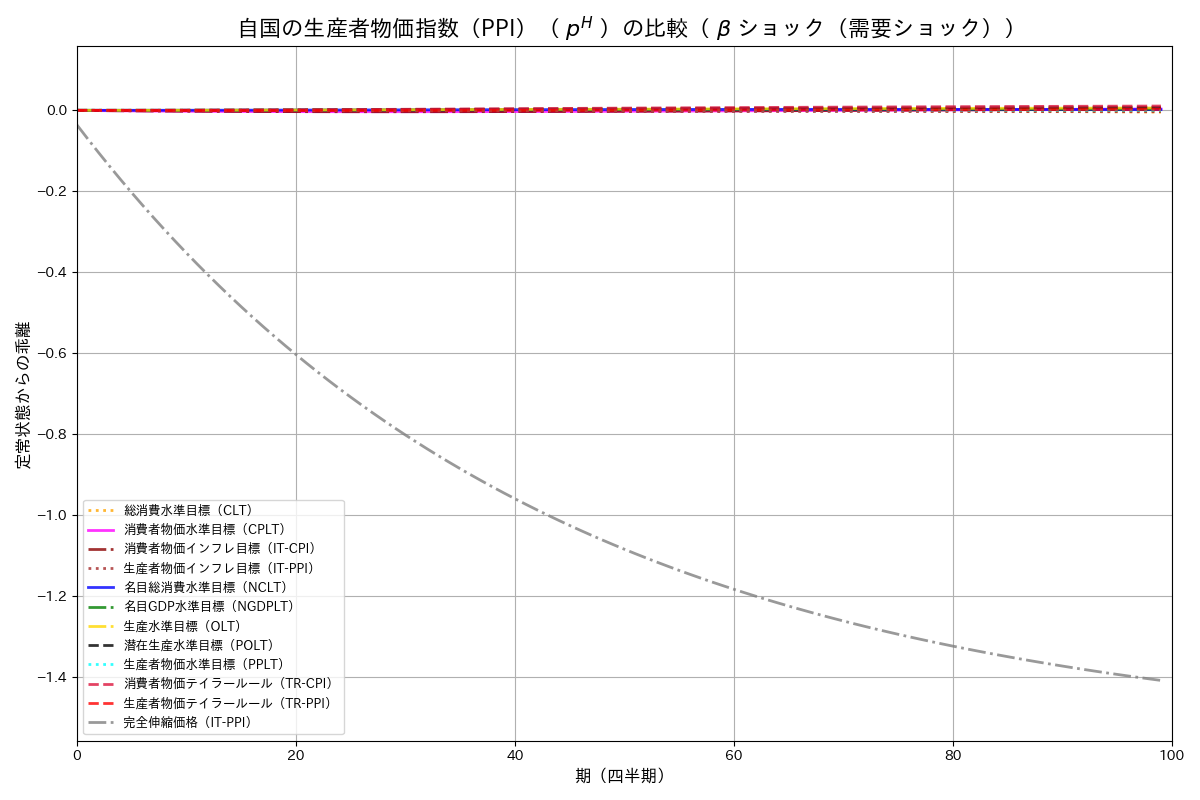
\includegraphics[width=0.9\textwidth]{comparison_graphs/beta_shock/beta_shock_p_H.png}
    \caption{自国の生産者物価指数（PPI）\(p^H\)}
    \label{fig:chapter5_beta_shock_graphs_p_H}
\end{figure}
\begin{figure}[H]
    \centering
    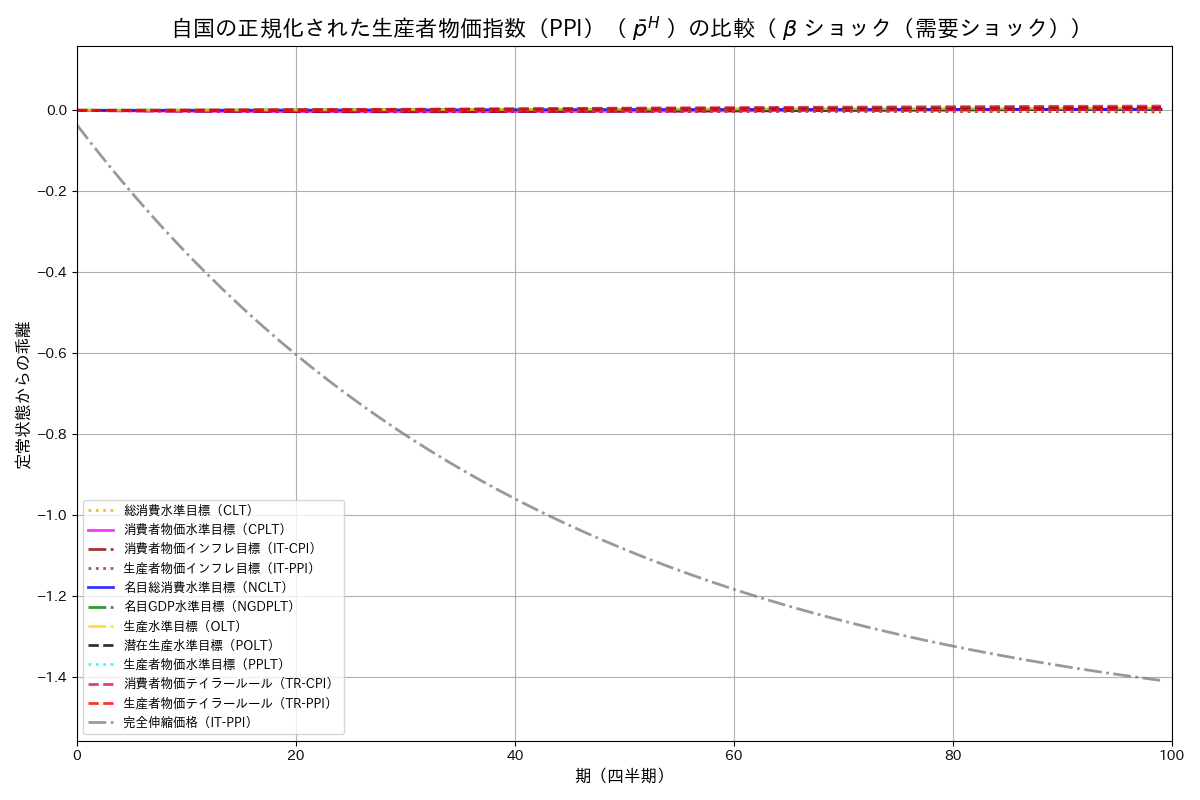
\includegraphics[width=0.9\textwidth]{comparison_graphs/beta_shock/beta_shock_p_H_bar.png}
    \caption{自国の正規化された生産者物価指数（PPI）\(\bar{p}^H\)}
    \label{fig:chapter5_beta_shock_graphs_p_H_bar}
\end{figure}
\begin{figure}[H]
    \centering
    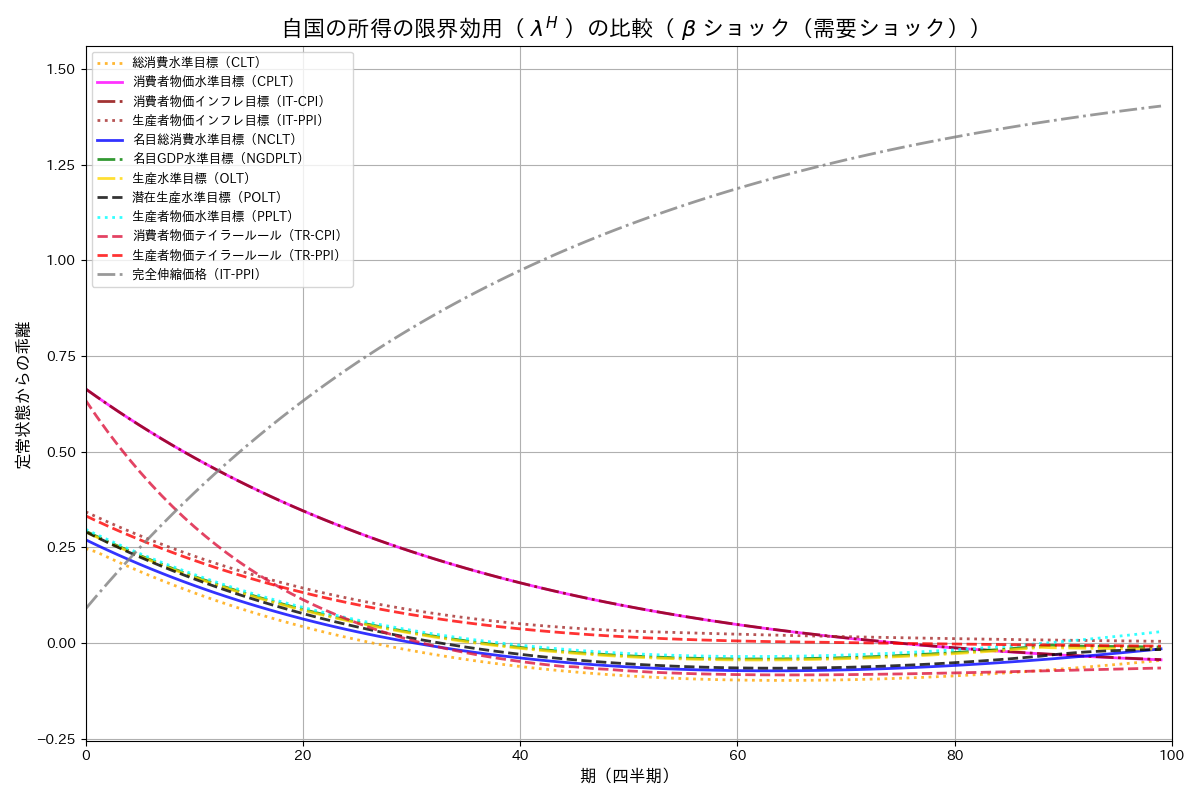
\includegraphics[width=0.9\textwidth]{comparison_graphs/beta_shock/beta_shock_lambda_H.png}
    \caption{自国の所得の限界効用\(\lambda^H\)}
    \label{fig:chapter5_beta_shock_graphs_lambda_H}
\end{figure}
\begin{figure}[H]
    \centering
    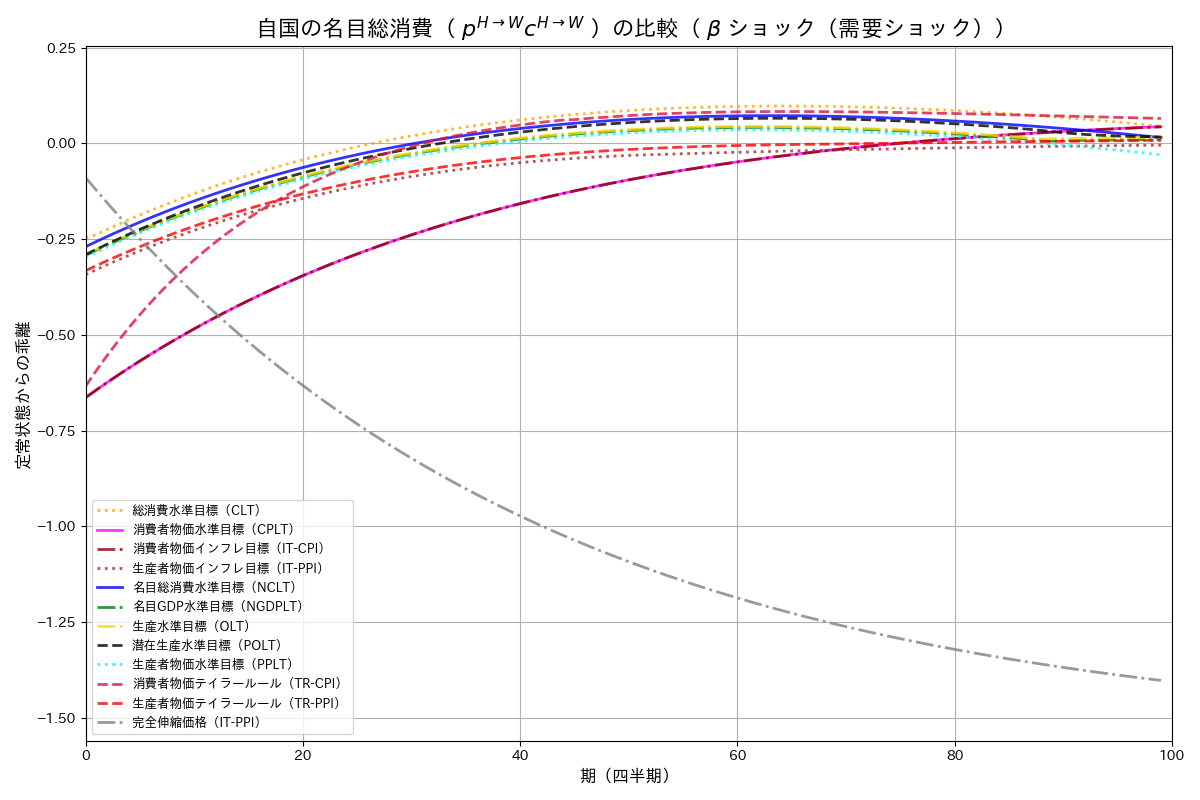
\includegraphics[width=0.9\textwidth]{comparison_graphs/beta_shock/beta_shock_p_H_W_c_H_W.png}
    \caption{自国の名目総消費\(p^{H\to W}c^{H\to W}\)}
    \label{fig:chapter5_beta_shock_graphs_p_H_W_c_H_W}
\end{figure}
\begin{figure}[H]
    \centering
    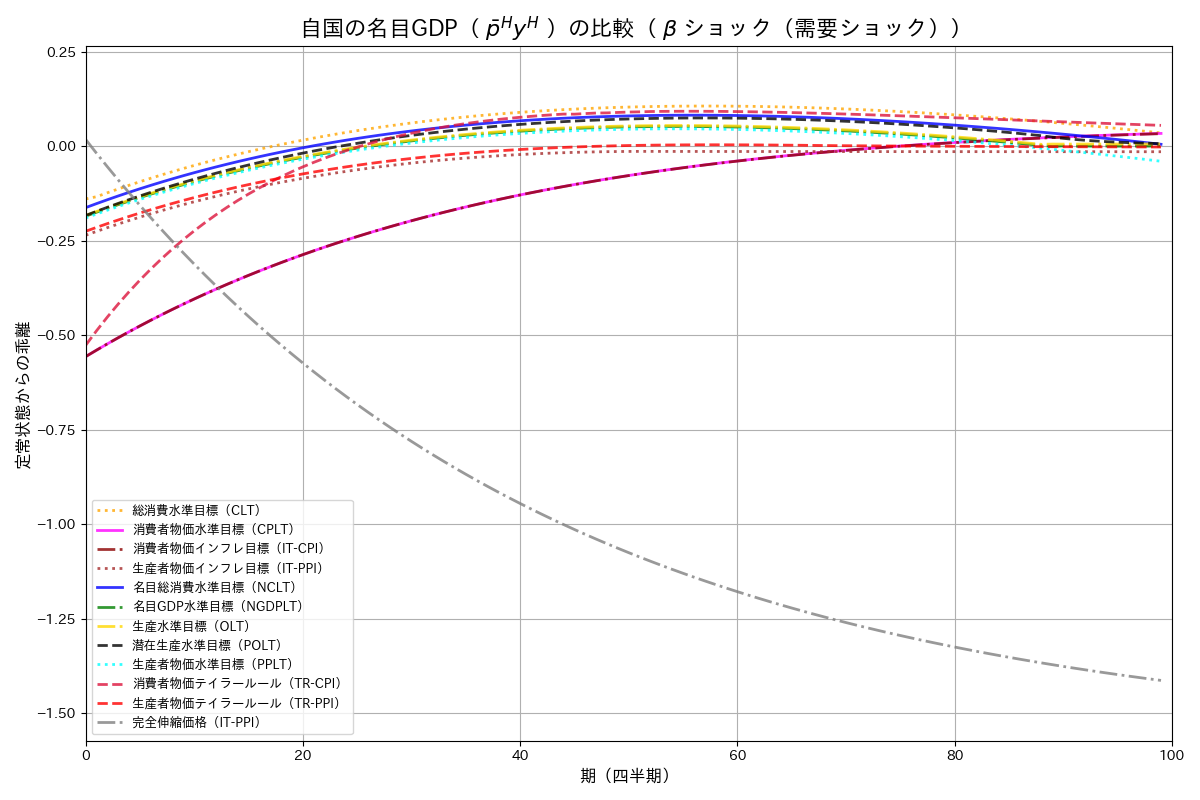
\includegraphics[width=0.9\textwidth]{comparison_graphs/beta_shock/beta_shock_p_H_bar_y_H.png}
    \caption{自国の名目GDP\(\bar{p}^Hy^H\)}
    \label{fig:chapter5_beta_shock_graphs_p_H_bar_y_H}
\end{figure}
\begin{figure}[H]
    \centering
    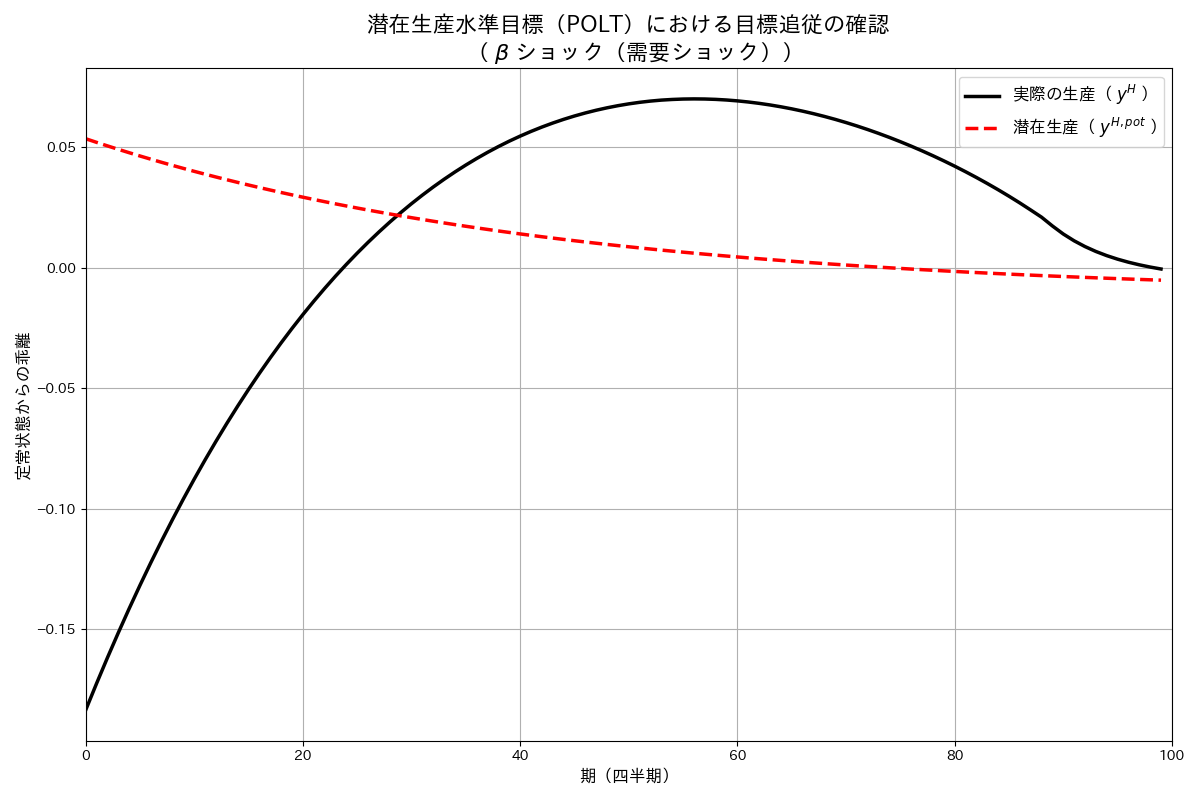
\includegraphics[width=0.9\textwidth]{comparison_graphs/beta_shock/beta_shock_polt_y_H_and_y_H_potential.png}
    \caption{自国の生産\(y^H\)と潜在生産\(y^{H,pot}\)潜在生産水準目標}
    \label{fig:chapter5_beta_shock_graphs_y_H_potential}
\end{figure}
\begin{figure}[H]
    \centering
    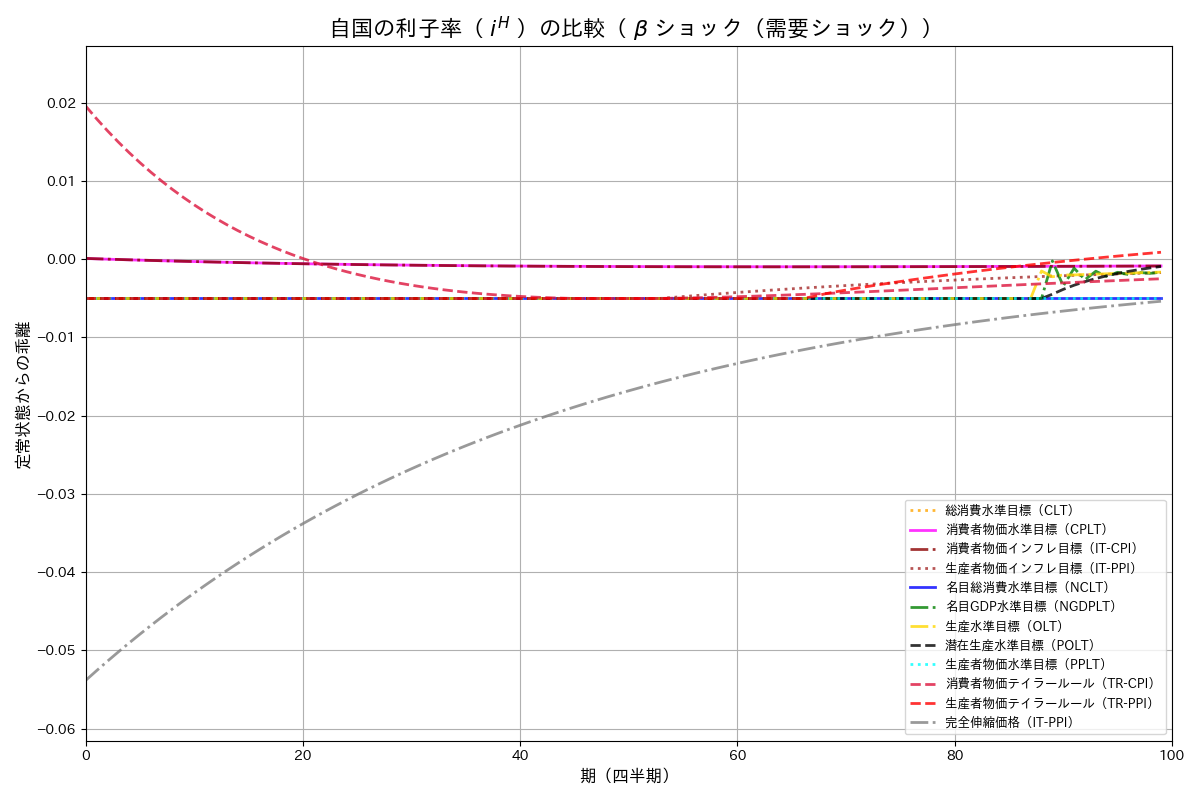
\includegraphics[width=0.9\textwidth]{comparison_graphs/beta_shock/beta_shock_i_H.png}
    \caption{自国の名目利子率\(i^H\)}
    \label{fig:chapter5_beta_shock_graphs_i_H}
\end{figure}
\begin{figure}[H]
    \centering
    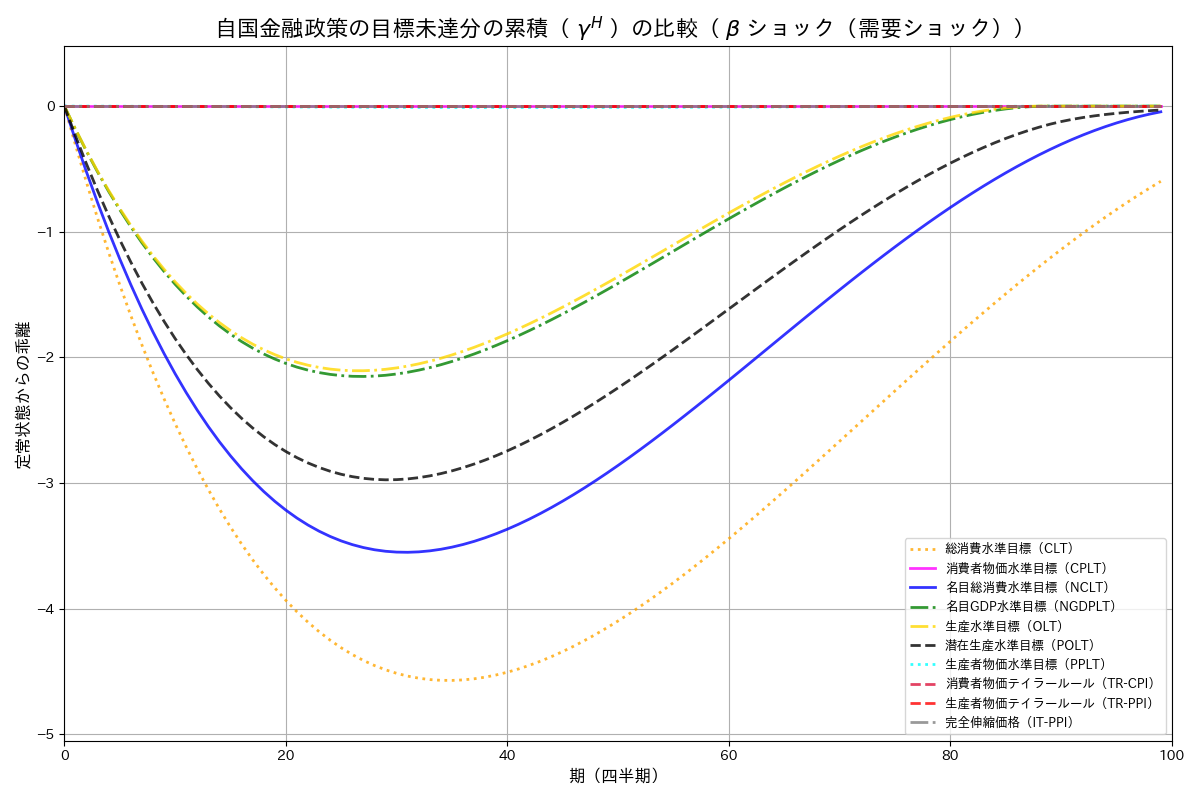
\includegraphics[width=0.9\textwidth]{comparison_graphs/beta_shock/beta_shock_gamma_H.png}
    \caption{自国の目標未達分の累積\(\gamma^H\)}
    \label{fig:chapter5_beta_shock_graphs_gamma_H}
\end{figure}